\documentclass[]{elsarticle}
%\documentclass[review]{elsarticle}

\usepackage{lineno,hyperref}
\modulolinenumbers[2]

\journal{Remote Sensing of Environment}

%%%%%%%%%%%%%%%%%%%%%%%
%% Elsevier bibliography styles
%%%%%%%%%%%%%%%%%%%%%%%
%% To change the style, put a % in front of the second line of the current style and
%% remove the % from the second line of the style you would like to use.
%%%%%%%%%%%%%%%%%%%%%%%

%% Numbered
%\bibliographystyle{model1-num-names}

%% Numbered without titles
%\bibliographystyle{model1a-num-names}

%% Harvard
%\bibliographystyle{model2-names.bst}\biboptions{authoryear}

%% Vancouver numbered
%\usepackage{numcompress}\bibliographystyle{model3-num-names}

%% Vancouver name/year
%\usepackage{numcompress}\bibliographystyle{model4-names}\biboptions{authoryear}

%% APA style
%\bibliographystyle{model5-names}\biboptions{authoryear}

%% AMA style
%\usepackage{numcompress}\bibliographystyle{model6-num-names}

%% `Elsevier LaTeX' style
\bibliographystyle{elsarticle-num}
%%%%%%%%%%%%%%%%%%%%%%%

\begin{document}

\begin{frontmatter}

\title{Understanding the drivers of diurnal and nocturnal urban land surface temperature}

%% or include affiliations in footnotes:
\author[1]{T.M. Logan\corref{mycorrespondingauthor}}
\cortext[mycorrespondingauthor]{Corresponding author}
\ead[url]{www.tomlogan.co.nz}
\ead{tomlogan@umich.edu}

\author[2]{B. Zaitchik}
\author[1]{S. Guikema}


\address[1]{Industrial and Operations Engineering, University of Michigan, Ann Arbor, MI}
\address[2]{Earth and Planetary Sciences, Johns Hopkins University, Baltimore, MD}

\begin{abstract}
Understanding the drivers of urban land thermal radiance, a key factor of land surface temperature, can assist in ameliorating the severity of the urban heat island and risk from heat waves. Of all the natural events, heat waves are among the deadliest and are likely to become longer and more frequent with climatic changes. Coupled with demographic shifts towards urban living, climate change puts significant impetus on reducing community exposure to heat waves. An understudied aspect of urban land surface temperature is factors related to nocturnal surface temperature. Nocturnal land surface temperature is important in heat wave mitigation given the urban heat island effect is most apparent during the night and the minimum nocturnal temperature is linked with heat stress and mortality. In this study, we examine the day and night urban land surface temperature (with Landsat) in seven cities across the United States. We test a series of hypotheses regarding the effect of greenspace, water bodies, and impervious surfaces on land surface temperature using advanced statistical methods. The robustness of these results is tested using different cities and satellite imagery and the results of diurnal and nocturnal analysis are compared to determine if the expected relationships hold throughout the day and night. Understanding whether the factors related to high urban temperatures are consistent across US cities is important for climate adaptation planning and capable predictive models suggest the potential for analysing the effect of potential biophysical changes might have on land surface temperature.
\end{abstract}

\begin{keyword}

\end{keyword}

\end{frontmatter}

\linenumbers

\section{Introduction}


\section{Data and Methods}


\section{Results and Discussion}

\subsection{Variables related to Land Surface Temperature}


\begin{figure}[h]
\begin{center}
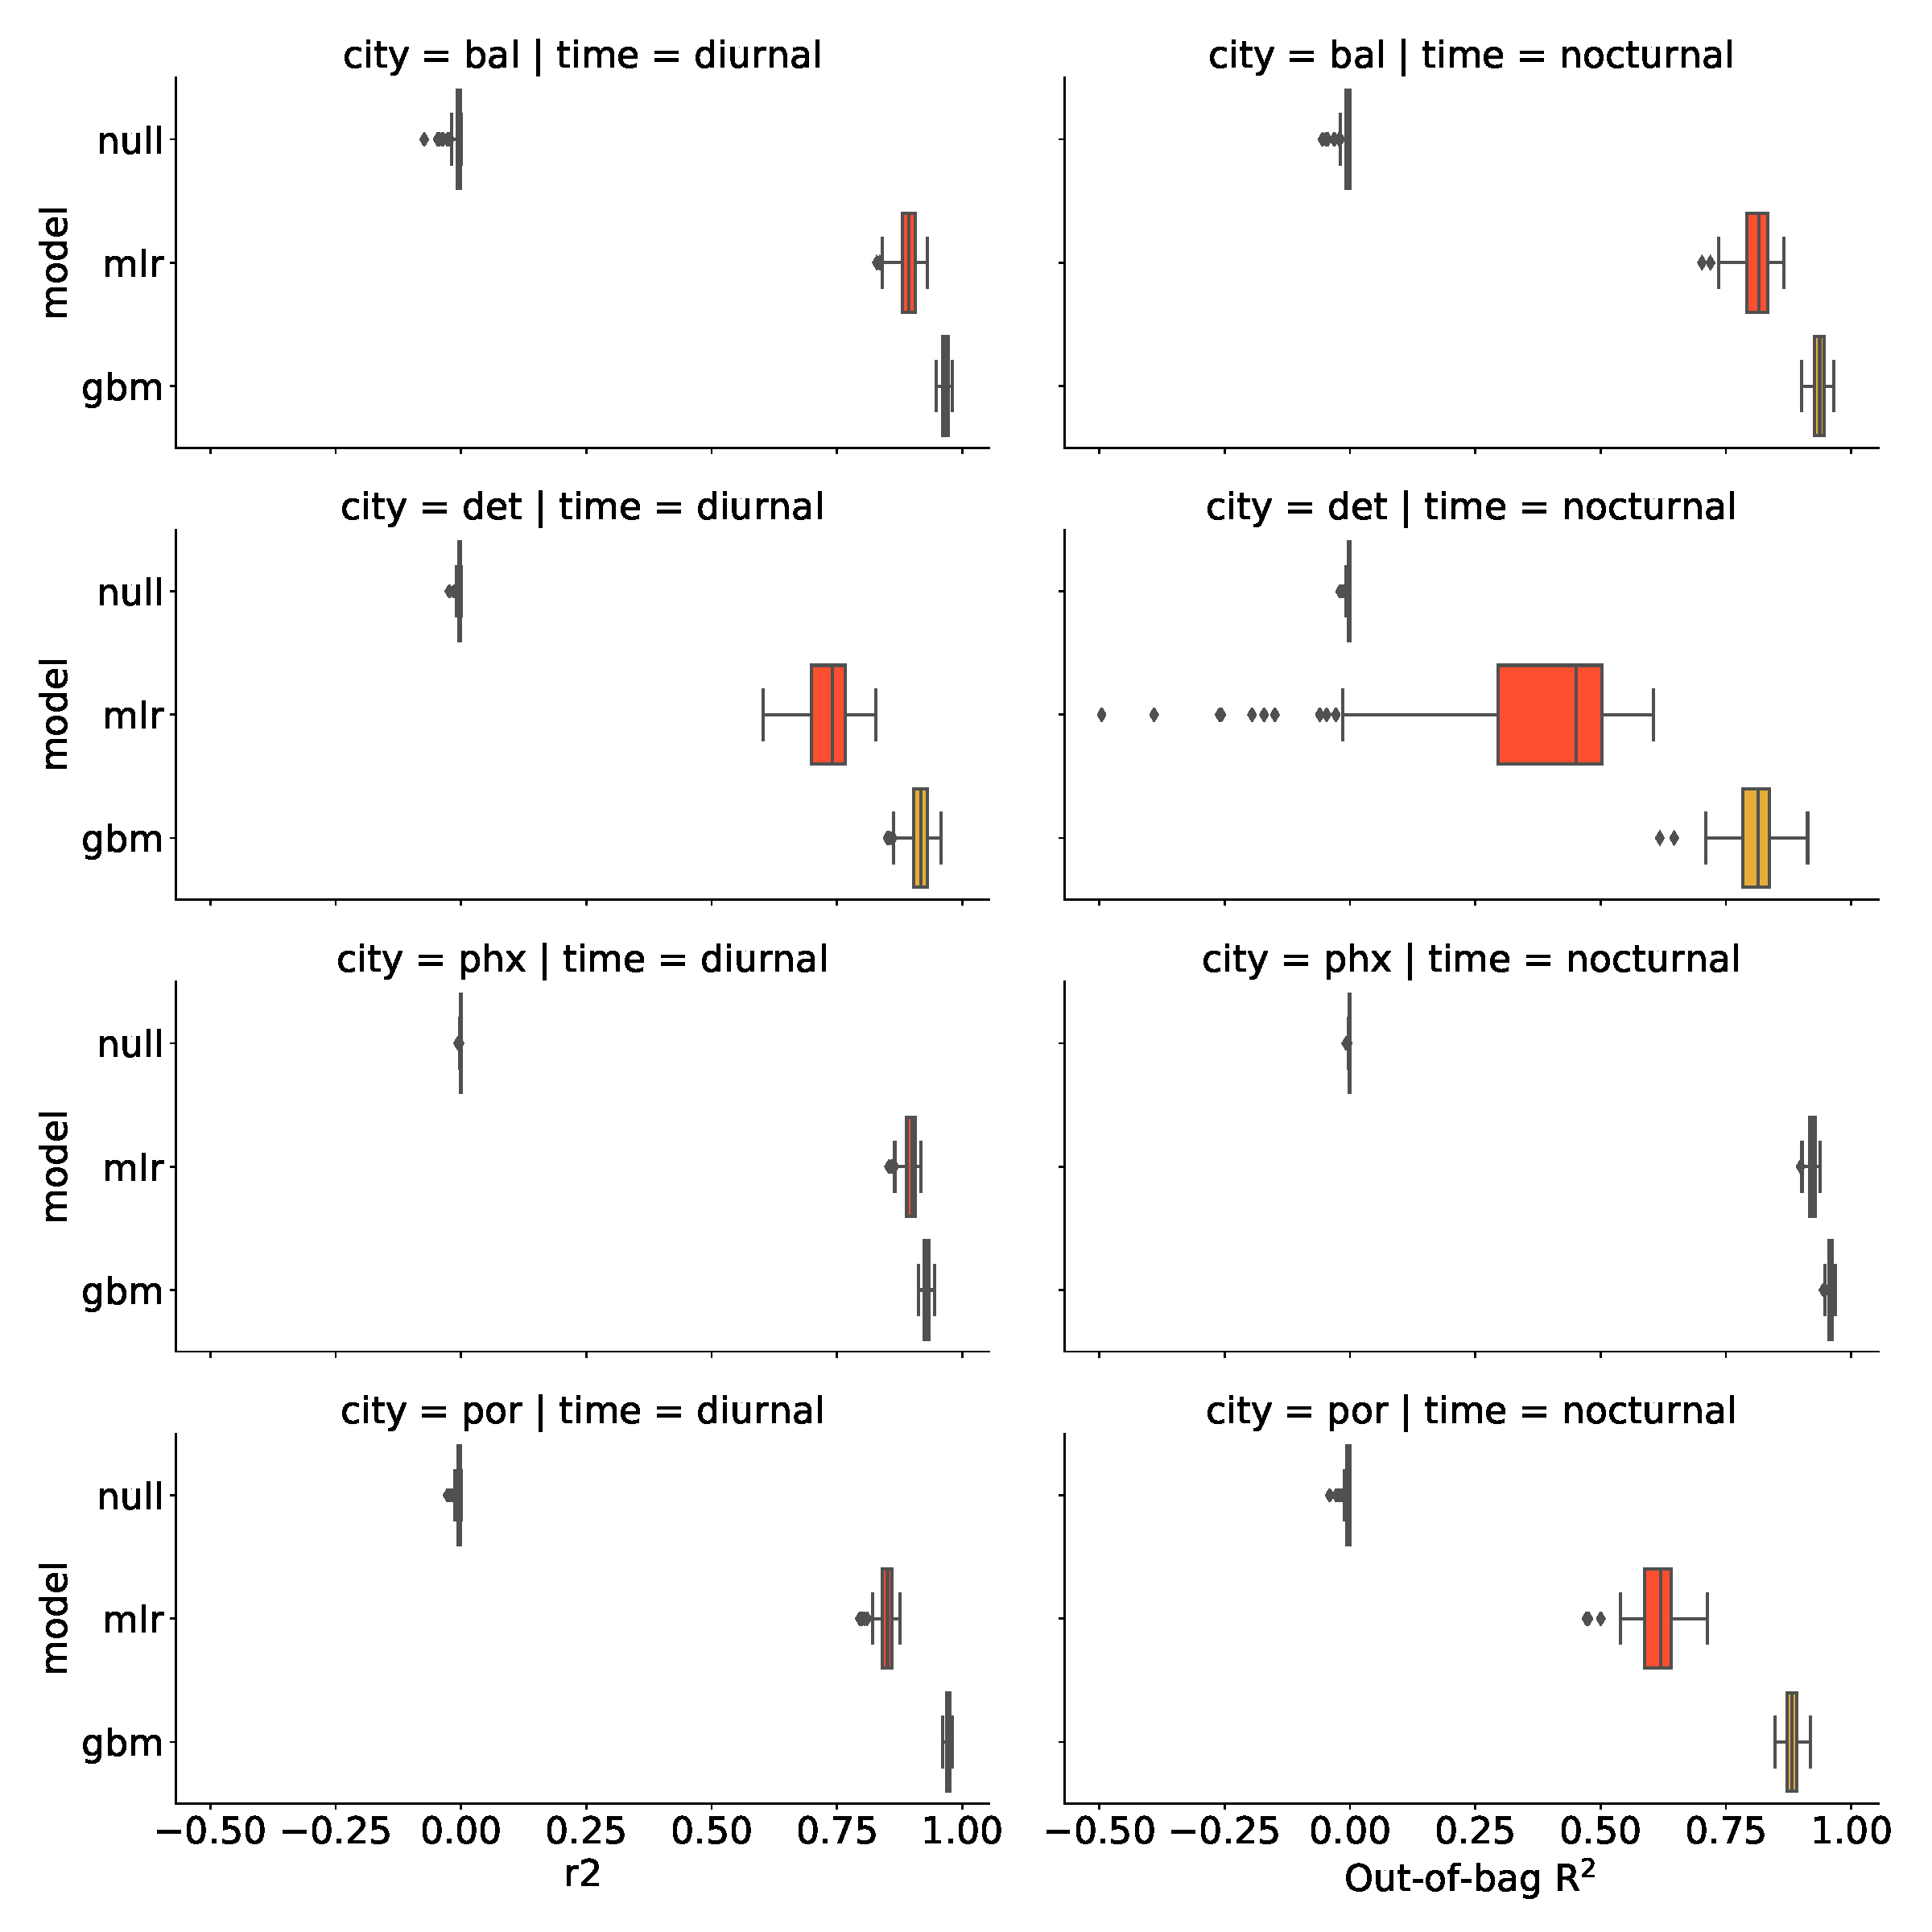
\includegraphics[width=\textwidth]{fig/report/holdout_results_r2.pdf}
\caption{The out-of-bag R$^2$ of the models when fitted on each city and used to predict a random sample from the same city. Out-of-bag R$^2$ can vary between $(-\infty, 1)$, where better models have a value near 1. This shows that the gradient boosted regression forest (gbm) consistently outperforms the multiple linear regression and null models.}
\label{fig:cityholdout_errors}
\end{center}
\end{figure}


\subsection{Predicting Land Surface Temperature Between Cities}

\begin{figure}[h]
\begin{center}
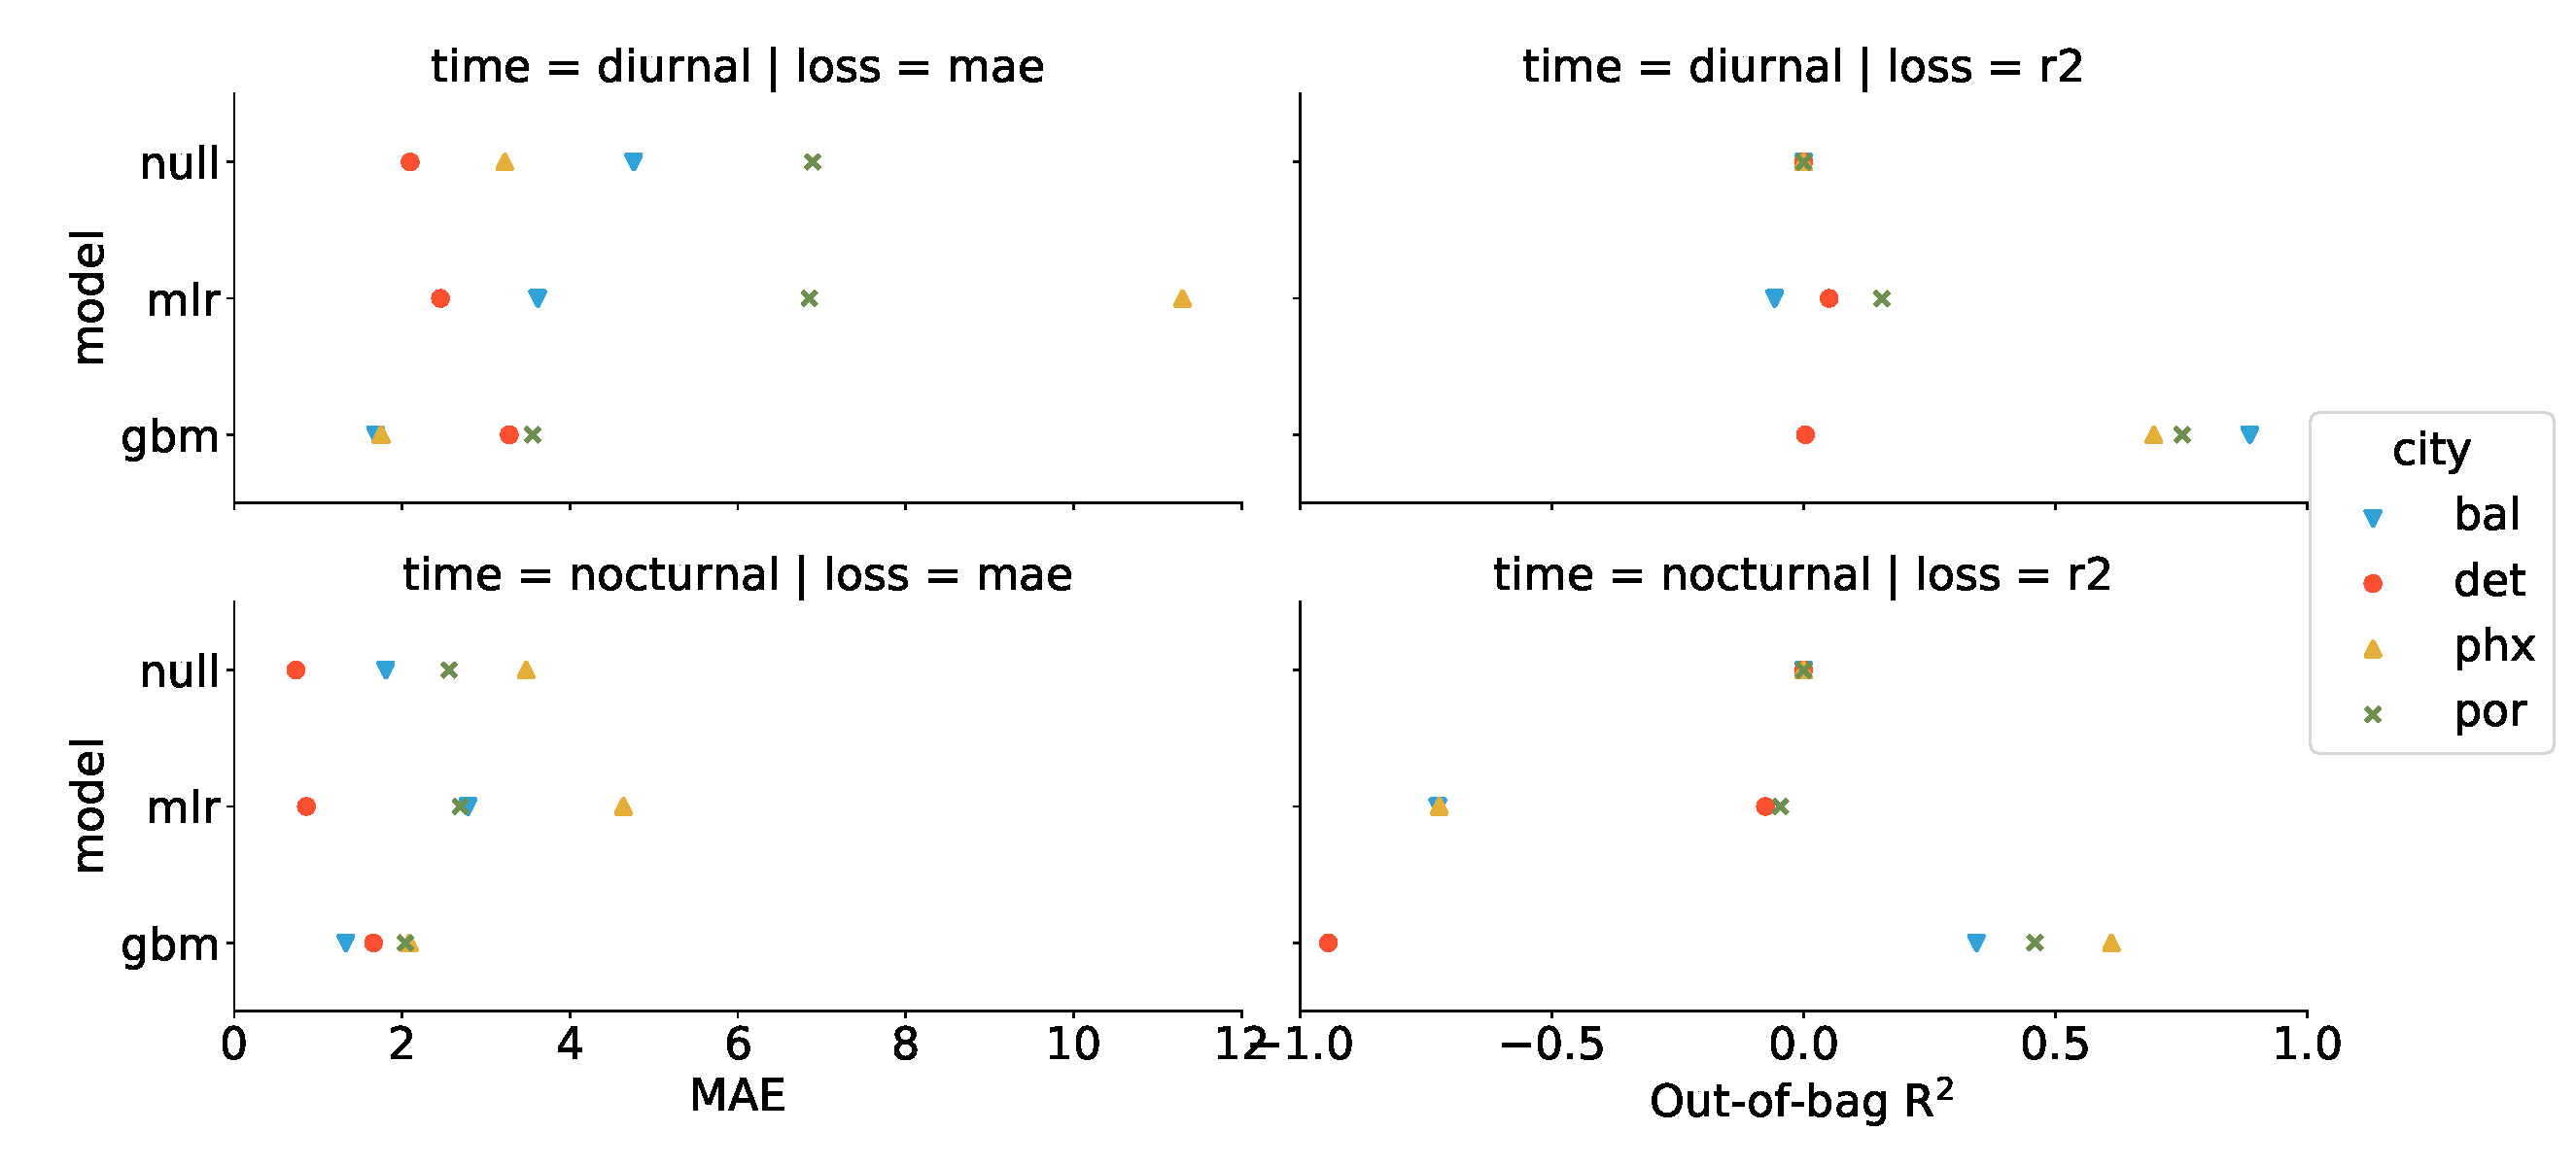
\includegraphics[width=\textwidth]{fig/report/cities_holdout.pdf}
\caption{The out-of-bag (OOB) R$^2$ and mean absolute error (MAE) of the models when fitted on three of the four cities and then used to predict the remaining city. OOB R$^2$ can vary between $(-\infty, 1)$, where better models have a value near 1. Good models have MAE near 0. The gradient boosted regression forest generally outperforms the other models, except when predicting Detroit. Note that the R$^2$ axis is truncated at -1, although the multiple linear regression for diurnal land surface temperature tested on Phoenix has an OOB R$^2$ of -9.  This shows that the gradient boosted regression forest (gbm) consistently outperforms the multiple linear regression and null models.}
\label{fig:cityholdout_errors}
\end{center}
\end{figure}


\section{Conclusion}

There are various bibliography styles available. You can select the style of your choice in the preamble of this document. These styles are Elsevier styles based on standard styles like Harvard and Vancouver. Please use Bib\TeX\ to generate your bibliography and include DOIs whenever available.

Here are two sample references: \cite{Feynman1963118,Dirac1953888}.

\section*{References}

\bibliography{mybibfile}

\appendix
\section{2013 Land Surface Temperature Image}


\section{Additional model results}
\begin{figure}[h]
\begin{center}
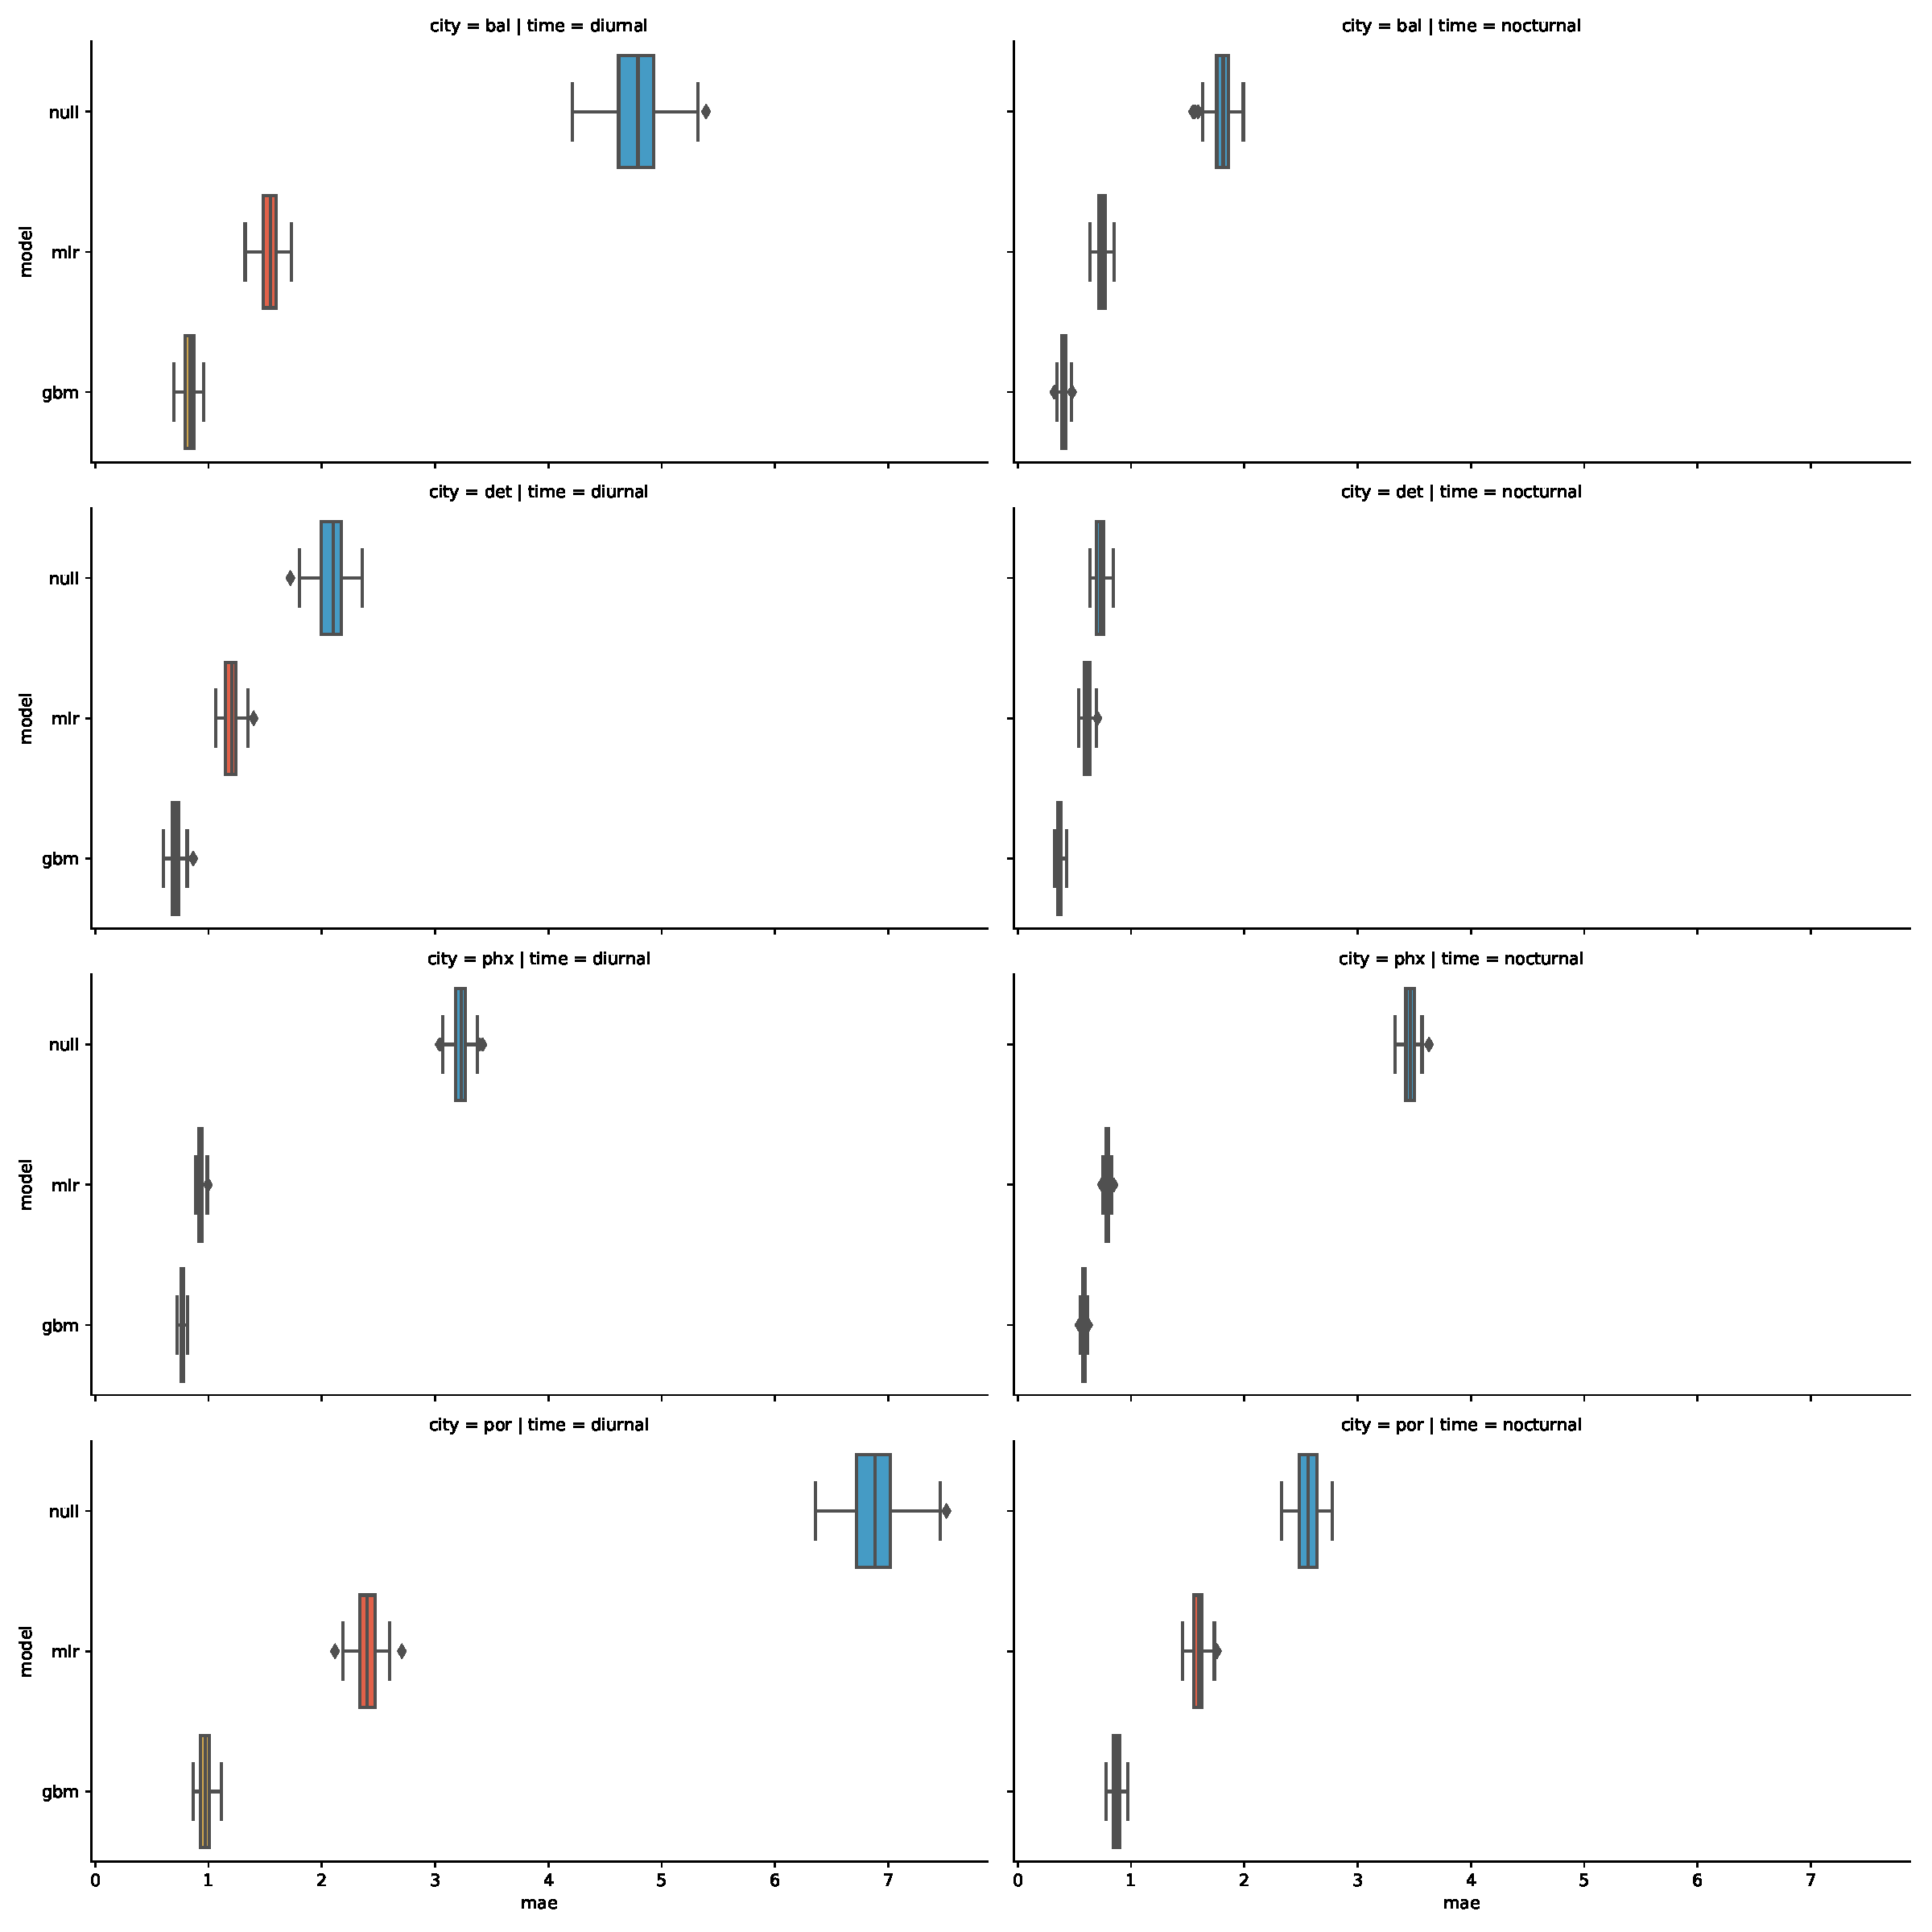
\includegraphics[width=\textwidth]{fig/report/holdout_results_mae.pdf}
\caption{The Mean Absolute Error (MAE) in $^oC$ of the models when fitted on each city and used to predict a random sample from the same city. Better models have lower MAE. This shows that the gradient boosted regression forest (gbm) consistently outperforms the multiple linear regression and null models. }
\label{fig:cityholdout_errors}
\end{center}
\end{figure}




\end{document}